%%%%%%%%%%%%%%%%%%%%%%%%%%%%%%%%%%%%%%%%%%%%%%%%%%%%%%%%%%%%%%%%%%%%%%%%%%%%%%%%
\chapter{Telecom RAG Assistant}
\label{chap:telecom_rag}

The Telecom Retrieval-Augmented Generation (RAG) Assistant is one of the four intelligent modules developed within the RANPilotAI platform. It is designed to assist Radio Access Network (RAN) engineers in efficiently retrieving and understanding information from official Third Generation Partnership Project (3GPP) Technical Specifications. Unlike conventional AI chatbots that rely solely on the internal knowledge of Large Language Models (LLMs), the proposed assistant integrates semantic retrieval with language generation, ensuring that every generated response is grounded in authentic engineering documentation.

The assistant combines document preprocessing, semantic chunking, dense embedding generation, vector similarity search, neural re-ranking, prompt engineering, and Large Language Models into a unified Retrieval-Augmented Generation pipeline. Consequently, engineers can ask technical questions using natural language while receiving structured responses supported by direct citations from the corresponding 3GPP specifications.

%%%%%%%%%%%%%%%%%%%%%%%%%%%%%%%%%%%%%%%%%%%%%%%%%%%%%%%%%%%%%%%%%%%%%%%%%%%%%%%%
\section{Introduction}

Modern LTE and 5G New Radio (NR) networks are standardized by hundreds of Technical Specifications published by the Third Generation Partnership Project (3GPP). These specifications define every aspect of the cellular system, including Radio Resource Control (RRC), Packet Data Convergence Protocol (PDCP), Radio Link Control (RLC), Medium Access Control (MAC), mobility management, measurement procedures, bearer configuration, security mechanisms, and radio resource management.

Although these documents serve as the authoritative engineering reference, they collectively contain thousands of pages distributed across multiple releases and specification documents. Locating a specific protocol definition, signaling procedure, configuration parameter, or ASN.1 structure often requires manually searching several PDF files and navigating numerous sections before identifying the required information. Traditional keyword-based searching is inefficient because engineering concepts are frequently distributed across different chapters, tables, annexes, and protocol descriptions.

Recent advances in Large Language Models (LLMs) have significantly improved natural language interaction with technical information. However, general-purpose language models cannot be considered authoritative engineering references because they generate responses solely from learned knowledge and may therefore produce inaccurate or hallucinated technical information. Such inaccuracies are unacceptable in professional telecommunication environments where engineering decisions must comply with official standards.

To address these challenges, the proposed Telecom RAG Assistant employs a Retrieval-Augmented Generation architecture. Rather than generating answers directly from the language model, the system first retrieves the most relevant sections from locally indexed 3GPP specifications before constructing the prompt supplied to the LLM. This approach combines the reasoning capabilities of modern language models with the reliability of official technical documentation, producing responses that are both accurate and traceable.

The Telecom RAG Assistant is fully integrated into the RANPilotAI platform alongside the KPI Degradation Analyzer, KPI Forecaster, and Optimization Action Analyzer. The platform provides a unified environment in which engineers can perform network analysis and standards consultation without switching between multiple software applications.

Figure~\ref{fig:rag_home} presents the main interface of the Telecom RAG Assistant. The interface enables engineers to select the RAG module, optionally restrict the search to a specific Technical Specification, submit engineering questions using natural language, and receive structured answers supported by citations extracted from the original specifications.

\begin{figure}[H]
    \centering
    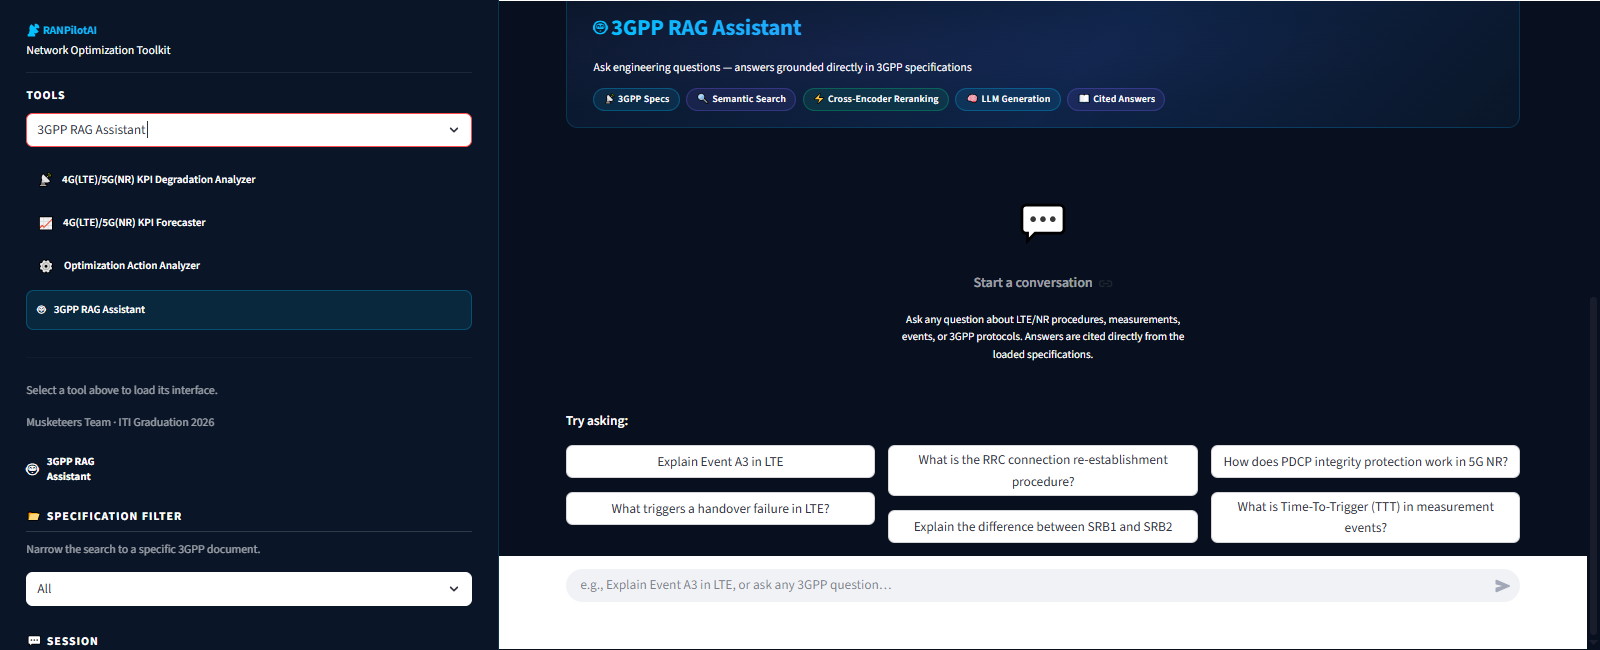
\includegraphics[width=\textwidth]{figures/chapter07/11.png}
    \caption{Main interface of the Telecom RAG Assistant integrated into the RANPilotAI platform. The interface provides access to the Telecom RAG module, allows filtering by specific 3GPP Technical Specifications, and supports interactive engineering question answering using Retrieval-Augmented Generation.}
    \label{fig:rag_home}
\end{figure}

Unlike conventional document search systems, the developed assistant performs semantic understanding of both the user's query and the indexed specification content. Consequently, relevant information can be retrieved even when the wording used by the engineer differs from the terminology employed within the official specification.

Furthermore, the generated responses are presented in a structured and readable format that includes hierarchical headings, explanatory paragraphs, engineering tables, bullet lists, and expandable citation panels. This presentation enables engineers not only to obtain concise explanations but also to verify every statement against the corresponding sections of the official 3GPP documentation.

%%%%%%%%%%%%%%%%%%%%%%%%%%%%%%%%%%%%%%%%%%%%%%%%%%%%%%%%%%%%%%%%%%%%%%%%%%%%%%%%
\section{Motivation}

Radio Access Network engineers routinely consult 3GPP Technical Specifications during network optimization, protocol analysis, interoperability testing, feature implementation, and troubleshooting activities. As LTE and 5G technologies continue to evolve, the complexity of these specifications has increased substantially, introducing thousands of configurable parameters, signaling procedures, optional features, and release-specific enhancements.

In traditional engineering workflows, locating the required information often involves opening multiple PDF documents, performing repetitive keyword searches, comparing several specification releases, and manually interpreting protocol descriptions before obtaining a complete understanding of the desired concept. This process is both time-consuming and inefficient, particularly when information is distributed across multiple sections or Technical Specifications.

Although modern Large Language Models provide an intuitive conversational interface, they cannot guarantee engineering accuracy because they do not inherently reference official standards during inference. Consequently, generated responses may contain incomplete explanations, outdated information, or fabricated protocol behavior. Such limitations significantly reduce their reliability for standards-based engineering applications.

The primary motivation behind developing the Telecom RAG Assistant was therefore to combine the natural language understanding capabilities of modern LLMs with the reliability of official 3GPP specifications. By integrating semantic retrieval with language generation, the assistant ensures that every response is generated using authentic engineering context retrieved directly from the indexed documents.

Another important objective was to reduce the time required for standards consultation. Instead of manually navigating hundreds of pages across multiple specifications, engineers can simply submit questions in natural language and immediately receive concise technical explanations accompanied by explicit references to the corresponding Technical Specification, release version, section number, and page number.

The developed graphical interface further enhances usability by allowing users to restrict searches to specific Technical Specifications through the Specification Filter, observe the internal execution stages of the Retrieval-Augmented Generation pipeline, and review supporting citations for every generated response. This transforms static technical documentation into an interactive engineering assistant capable of supporting daily telecommunication engineering activities.
%%%%%%%%%%%%%%%%%%%%%%%%%%%%%%%%%%%%%%%%%%%%%%%%%%%%%%%%%%%%%%%%%%%%%%%%%%%%%%%%
\section{Problem Statement}

The exponential growth of LTE and 5G New Radio (NR) standards has significantly increased the complexity of engineering documentation. Modern 3GPP Technical Specifications consist of thousands of pages describing protocol procedures, signaling messages, configuration parameters, ASN.1 definitions, state machines, timers, and implementation guidelines. Although these documents serve as the official reference for telecommunication systems, efficiently locating the required information remains a major challenge for network engineers.

Traditional document retrieval techniques rely primarily on keyword-based searches within Portable Document Format (PDF) files. While these methods are suitable for locating exact phrases, they frequently fail when users employ different terminology or when the required information is distributed across multiple specification sections. For example, an engineer searching for "Why is the HO-Conn field required?" may not retrieve the relevant specification if the document describes the same concept using formal protocol terminology rather than the user's wording.

General-purpose Large Language Models provide an alternative approach by enabling natural language interaction with technical knowledge. However, these models generate responses based on their internal parameters rather than official engineering references. Consequently, they may produce inaccurate explanations, outdated information, or fabricated protocol descriptions. Such hallucinations are unacceptable in professional telecommunication environments where engineering decisions must strictly comply with standardized specifications.

Therefore, the primary challenge addressed in this work is the development of an intelligent question-answering system capable of combining semantic understanding with authoritative document retrieval. The system should allow engineers to interact with 3GPP specifications using natural language while ensuring that every generated response remains grounded in authentic engineering documentation.

To address this challenge, the proposed Telecom RAG Assistant employs a Retrieval-Augmented Generation (RAG) architecture that retrieves the most relevant specification sections before generating the final response. This approach significantly improves factual accuracy while preserving complete traceability to the original Technical Specifications.

%%%%%%%%%%%%%%%%%%%%%%%%%%%%%%%%%%%%%%%%%%%%%%%%%%%%%%%%%%%%%%%%%%%%%%%%%%%%%%%%
\section{Background}

The Telecom RAG Assistant integrates several modern Artificial Intelligence and Information Retrieval technologies to transform static engineering documentation into an interactive knowledge assistant. This section introduces the fundamental concepts that form the basis of the proposed system.

%%%%%%%%%%%%%%%%%%%%%%%%%%%%%%%%%%%%%%%%%%%%%%%%%%%%%%%%%%%%%%%%%%%%%%%%%%%%%%%%
\subsection{Large Language Models (LLMs)}

Large Language Models (LLMs) are deep neural networks trained on massive textual datasets to predict the next token in a sequence. Modern LLMs are primarily based on the Transformer architecture, which employs self-attention mechanisms to capture long-range dependencies between words and sentences.

Recent models such as GPT, LLaMA, Claude, Gemini, and DeepSeek have demonstrated remarkable capabilities in natural language understanding, reasoning, summarization, translation, and conversational question answering. These capabilities enable users to interact with complex technical information using natural language instead of predefined commands or structured queries.

Despite their impressive performance, LLMs suffer from several limitations when applied to engineering applications. Since their knowledge is acquired during training, newly published standards or updated technical documents cannot be accessed unless the model is retrained. Furthermore, the generated responses may contain hallucinations, where the model produces fluent but factually incorrect information. In standards-based domains such as telecommunications, such inaccuracies may lead to incorrect engineering decisions.

Consequently, rather than relying exclusively on an LLM, the proposed system augments the language model with external knowledge retrieved directly from official 3GPP specifications.

%%%%%%%%%%%%%%%%%%%%%%%%%%%%%%%%%%%%%%%%%%%%%%%%%%%%%%%%%%%%%%%%%%%%%%%%%%%%%%%%
\subsection{Retrieval-Augmented Generation (RAG)}

Retrieval-Augmented Generation (RAG) is a hybrid Artificial Intelligence framework that combines document retrieval with neural language generation. Instead of generating responses solely from the model's internal knowledge, a RAG system first retrieves the most relevant documents from an external knowledge base and then incorporates these documents into the prompt supplied to the language model.

The general RAG workflow consists of four sequential stages:

\begin{enumerate}
    \item User query processing.
    \item Semantic retrieval of relevant document chunks.
    \item Prompt construction using the retrieved context.
    \item Response generation by the Large Language Model.
\end{enumerate}

This architecture provides several important advantages over standalone language models. First, it allows the knowledge base to be updated without retraining the language model. Second, it significantly reduces hallucinations because responses are generated using authentic supporting documents. Finally, it enables explicit citation of the retrieved sources, thereby improving transparency and user confidence.

Within the proposed Telecom RAG Assistant, Retrieval-Augmented Generation serves as the core framework that connects semantic search with natural language generation, enabling accurate engineering question answering over official 3GPP Technical Specifications.

%%%%%%%%%%%%%%%%%%%%%%%%%%%%%%%%%%%%%%%%%%%%%%%%%%%%%%%%%%%%%%%%%%%%%%%%%%%%%%%%
\subsection{Embedding Models}

Semantic retrieval requires transforming textual information into numerical representations that preserve contextual meaning. This transformation is performed using embedding models, which encode sentences or document passages into dense high-dimensional vectors.

Unlike traditional keyword matching, embedding models capture semantic similarity between different textual expressions. Consequently, two sentences describing the same engineering concept using different terminology are represented by nearby vectors in the embedding space.

For example, the following engineering questions express similar meanings despite using different wording:

\begin{itemize}
    \item What is Event A3?
    \item Explain the A3 measurement event.
    \item How does LTE Event A3 trigger handover?
\end{itemize}

A high-quality embedding model generates similar vector representations for these queries, enabling the retrieval engine to identify the same specification sections regardless of the exact wording used by the engineer.

The Telecom RAG Assistant employs a transformer-based embedding model to encode both the indexed specification chunks and incoming user queries into a shared semantic vector space.

%%%%%%%%%%%%%%%%%%%%%%%%%%%%%%%%%%%%%%%%%%%%%%%%%%%%%%%%%%%%%%%%%%%%%%%%%%%%%%%%
\subsection{Vector Databases}

After generating dense embeddings for every document chunk, an efficient mechanism is required to store and retrieve these vectors. Traditional relational databases are not designed for similarity search in high-dimensional vector spaces. Instead, specialized vector databases perform Approximate Nearest Neighbor (ANN) search to efficiently retrieve semantically similar vectors.

The proposed system utilizes Qdrant as the vector database responsible for storing all embedded document chunks together with their associated metadata. Besides the dense embeddings, each indexed record contains additional information including:

\begin{itemize}
    \item Technical Specification number.
    \item 3GPP Release version.
    \item Section identifier.
    \item Page number.
    \item Document title.
\end{itemize}

This metadata enables the system to filter search results according to user-selected specifications while preserving complete traceability to the original engineering documents.

%%%%%%%%%%%%%%%%%%%%%%%%%%%%%%%%%%%%%%%%%%%%%%%%%%%%%%%%%%%%%%%%%%%%%%%%%%%%%%%%
\subsection{Cross Encoder Re-ranking}

Although dense vector retrieval effectively identifies semantically related document chunks, the retrieved results may still include partially relevant passages. To improve retrieval precision, the proposed system performs a second-stage neural re-ranking process using a Cross Encoder model.

Unlike embedding models that independently encode queries and documents, Cross Encoders jointly process both inputs and compute a direct relevance score for each query-document pair. This enables the model to perform deeper semantic analysis and produce a more accurate ranking of candidate document chunks.

After the initial vector search retrieves the top candidate passages, the Cross Encoder evaluates each retrieved chunk, assigns a relevance score, and reorders the results accordingly. Only the highest-ranked chunks are subsequently included in the final prompt supplied to the language model.

This two-stage retrieval strategy combines the efficiency of vector similarity search with the accuracy of neural relevance estimation, significantly improving the quality of the generated engineering responses while minimizing irrelevant contextual information.
%%%%%%%%%%%%%%%%%%%%%%%%%%%%%%%%%%%%%%%%%%%%%%%%%%%%%%%%%%%%%%%%%%%%%%%%%%%%%%%%
\section{Overall System Architecture}

The Telecom RAG Assistant follows a modular Retrieval-Augmented Generation (RAG) architecture specifically designed for querying official 3GPP Technical Specifications. The architecture integrates document preprocessing, semantic indexing, vector retrieval, neural re-ranking, prompt construction, and Large Language Model (LLM) inference into a unified pipeline. Each module performs a dedicated task while interacting with adjacent modules through well-defined interfaces, resulting in a scalable and maintainable software architecture.

Unlike conventional document search systems, the proposed architecture performs semantic retrieval instead of keyword matching. Both the indexed specification documents and incoming user queries are represented as dense embedding vectors. Similarity search is then performed within the embedding space, enabling the retrieval of conceptually related information even when different terminology is used.

The overall architecture of the proposed Telecom RAG Assistant is illustrated in Figure~\ref{fig:overall_architecture}.

\begin{figure}[H]
    \centering
    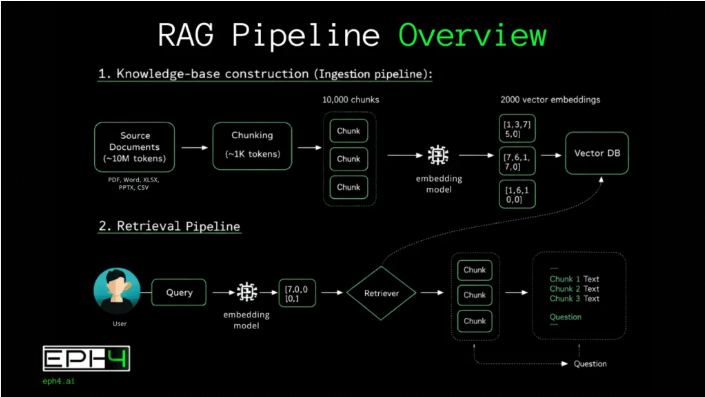
\includegraphics[width=0.95\textwidth]{figures/chapter07/RAG-Pipeline-How-RAG-Works-1024x576.png}
    \caption{Overall architecture of the proposed Telecom RAG Assistant.}
    \label{fig:overall_architecture}
\end{figure}

The complete system consists of the following processing stages:

\begin{enumerate}
    \item PDF Processing
    \item Section-aware Chunking
    \item Embedding Generation
    \item Vector Storage using Qdrant
    \item Metadata Filtering
    \item Dense Vector Retrieval
    \item Cross Encoder Re-ranking
    \item Prompt Construction
    \item LLM Response Generation
    \item Response Rendering with Source Citations
\end{enumerate}

Each module contributes to improving retrieval accuracy, reducing hallucination, and maintaining traceability to the original engineering documentation.

%%%%%%%%%%%%%%%%%%%%%%%%%%%%%%%%%%%%%%%%%%%%%%%%%%%%%%%%%%%%%%%%%%%%%%%%%%%%%%%%
\section{Software Architecture}

The Telecom RAG Assistant was implemented using a modular software architecture in which every component is responsible for a specific stage of the Retrieval-Augmented Generation pipeline. This modular design simplifies maintenance, facilitates future extensions, and allows individual components to be optimized independently.

The software architecture is composed of the following modules:

\begin{itemize}

\item \textbf{PDF Processing Module}

Extracts textual content and metadata from official 3GPP Technical Specifications.

\item \textbf{Section-aware Chunking Module}

Splits the extracted documents into semantically meaningful chunks while preserving the hierarchical structure of the specifications.

\item \textbf{Embedding Module}

Generates dense vector representations for every document chunk using the selected embedding model.

\item \textbf{Vector Database Module}

Stores all embedding vectors together with their associated metadata using the Qdrant vector database.

\item \textbf{Metadata Filtering Module}

Restricts document retrieval according to user-selected Technical Specifications.

\item \textbf{Retrieval Module}

Performs semantic similarity search to retrieve the Top-K most relevant document chunks.

\item \textbf{Cross Encoder Module}

Re-ranks the retrieved chunks according to their semantic relevance to the user query.

\item \textbf{Prompt Construction Module}

Builds the final prompt by combining the retrieved specification context with the user's question.

\item \textbf{Large Language Model Module}

Generates the final engineering response using the constructed prompt.

\item \textbf{Streamlit User Interface}

Provides the graphical interface through which users interact with the complete system.

\end{itemize}

The modular organization allows each subsystem to operate independently while contributing to the overall Retrieval-Augmented Generation workflow.

%%%%%%%%%%%%%%%%%%%%%%%%%%%%%%%%%%%%%%%%%%%%%%%%%%%%%%%%%%%%%%%%%%%%%%%%%%%%%%%%
\section{Query Processing Workflow}

The complete query processing workflow begins when the engineer submits a natural-language question through the Streamlit interface. Instead of directly forwarding the request to the Large Language Model, the proposed system executes a sequence of retrieval and validation stages to ensure that the generated response is based exclusively on relevant sections extracted from the indexed 3GPP specifications.

Figure~\ref{fig:query_pipeline} illustrates the execution stages displayed by the system while processing a user query.

\begin{figure}[H]
    \centering
    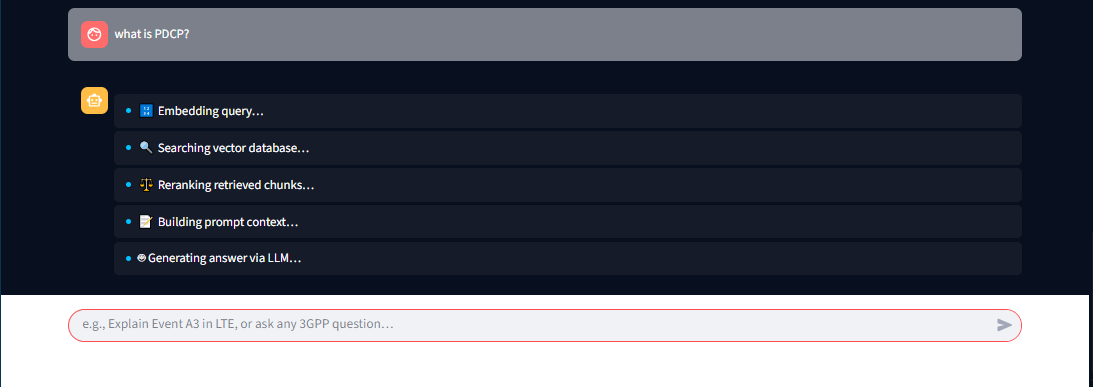
\includegraphics[width=\textwidth]{figures/chapter07/5.png}
    \caption{Real-time execution stages of the Retrieval-Augmented Generation pipeline during query processing.}
    \label{fig:query_pipeline}
\end{figure}

After receiving a user query, the system performs the following sequence of operations:

\begin{enumerate}

\item The user submits a technical question through the graphical interface.

\item The query is converted into a dense semantic embedding using the embedding model.

\item The generated embedding is submitted to the Qdrant vector database to retrieve the Top-K semantically similar document chunks.

\item Metadata filtering is applied whenever the user restricts the search to a specific Technical Specification.

\item Duplicate chunks are removed to maximize contextual diversity.

\item A Cross Encoder model evaluates each retrieved chunk and computes semantic relevance scores.

\item The highest-ranked chunks are selected to construct the final prompt.

\item The prompt is transmitted to the selected Large Language Model through the OpenRouter API.

\item The language model generates a structured engineering response based on the retrieved specification context.

\item Supporting citations are attached to the generated response, enabling engineers to verify every statement directly from the corresponding 3GPP Technical Specification.

\end{enumerate}

The graphical interface provides users with real-time feedback regarding the execution status of every processing stage, including embedding generation, vector retrieval, neural re-ranking, prompt construction, and response generation, thereby improving transparency and user confidence in the retrieval process.
%%%%%%%%%%%%%%%%%%%%%%%%%%%%%%%%%%%%%%%%%%%%%%%%%%%%%%%%%%%%%%%%%%%%%%%%%%%%%%%%
\section{PDF Processing}

The first stage of the proposed Telecom RAG Assistant consists of processing the official 3GPP Technical Specification documents. Since these specifications are distributed as Portable Document Format (PDF) files, their contents must first be transformed into a machine-readable representation before they can be indexed and queried.

Unlike conventional document parsers that simply extract plain text, the proposed system performs structured document analysis in order to preserve the hierarchical organization of the specifications. This is particularly important because 3GPP documents contain numbered sections, subsections, engineering tables, ASN.1 definitions, mathematical expressions, figures, and annexes, all of which contribute to the semantic meaning of the document.

The PDF processing module is responsible for extracting textual content, removing unnecessary formatting artifacts, identifying section boundaries, extracting engineering tables, and collecting document metadata such as the Technical Specification number, release version, page number, and document title. These metadata elements are preserved throughout the indexing pipeline and later attached to every retrieved chunk, allowing engineers to trace generated responses back to their original source.

The implementation utilizes the PyMuPDF library to efficiently parse PDF documents while preserving page-level information. During preprocessing, repetitive page headers, footers, and formatting artifacts are removed in order to improve retrieval quality. Engineering tables are detected and converted into Markdown representations, enabling the language model to interpret structured information more accurately than raw PDF text. This preprocessing stage significantly improves the readability and semantic consistency of the indexed documents.

The processed output generated by this stage serves as the input to the Section-aware Chunking module, which further organizes the extracted content into semantically meaningful units suitable for embedding generation.

%%%%%%%%%%%%%%%%%%%%%%%%%%%%%%%%%%%%%%%%%%%%%%%%%%%%%%%%%%%%%%%%%%%%%%%%%%%%%%%%
\section{Section-aware Chunking}

One of the most important contributions of the proposed Telecom RAG Assistant is the implementation of a section-aware chunking strategy specifically designed for 3GPP Technical Specifications.

Traditional Retrieval-Augmented Generation systems generally divide documents into fixed-size chunks based on a predefined number of tokens or characters. Although computationally simple, this approach frequently separates logically connected engineering concepts across multiple chunks. As a consequence, important contextual information may be lost, leading to incomplete retrieval results and reduced response quality.

To overcome this limitation, the developed system performs hierarchical chunking based on the structural organization of 3GPP specifications. Instead of splitting documents at arbitrary token boundaries, the chunking algorithm detects section headers, subsection identifiers, engineering tables, figure descriptions, annexes, ASN.1 definitions, and mathematical expressions. Each chunk therefore represents a complete engineering concept rather than an arbitrary text fragment.


\begin{itemize}
    \item The textual content extracted from the specification.
    \item Metadata describing the source Technical Specification, release version, section identifier, page number, and document type.
\end{itemize}

This structured representation enables subsequent retrieval stages to perform semantic search while simultaneously preserving complete traceability to the original engineering documentation.

%%%%%%%%%%%%%%%%%%%%%%%%%%%%%%%%%%%%%%%%%%%%%%%%%%%%%%%%%%%%%%%%%%%%%%%%%%%%%%%%
\section{Embedding Generation}

After document chunking has been completed, every chunk is transformed into a dense numerical representation using a transformer-based embedding model. These dense vectors capture the semantic meaning of each engineering concept, enabling similarity search beyond simple keyword matching.

The embedding model projects both specification chunks and incoming user queries into the same high-dimensional semantic vector space. Consequently, conceptually related texts are positioned close to one another regardless of the exact wording used. This capability enables engineers to formulate questions using natural language while still retrieving the appropriate specification sections.

During the indexing process, each document chunk is independently encoded before being inserted into the vector database. Similarly, every user query submitted through the graphical interface is encoded using the same embedding model. Since both document embeddings and query embeddings share the same semantic space, similarity can be efficiently computed using vector distance metrics.

The generated embeddings constitute the primary index used by the retrieval engine and form the foundation of the semantic search capabilities implemented within the Telecom RAG Assistant.

%%%%%%%%%%%%%%%%%%%%%%%%%%%%%%%%%%%%%%%%%%%%%%%%%%%%%%%%%%%%%%%%%%%%%%%%%%%%%%%%
\section{Vector Database (Qdrant)}

Following embedding generation, all dense vectors are stored inside a local Qdrant vector database. Qdrant was selected due to its efficient Approximate Nearest Neighbor (ANN) search algorithms, support for metadata filtering, lightweight deployment model, and seamless integration with Python-based machine learning frameworks.

Unlike cloud-hosted vector databases, the developed system employs Qdrant in embedded local mode. Consequently, the complete vector database resides on the local machine, eliminating external dependencies while improving data privacy and reducing deployment complexity.

Each indexed record stored within Qdrant contains both the embedding vector and its associated metadata. Typical metadata include:

\begin{itemize}
    \item Technical Specification number
    \item 3GPP Release version
    \item Section identifier
    \item Page number
    \item Document title
\end{itemize}

The inclusion of metadata enables advanced filtering operations during retrieval while preserving direct references to the original engineering documentation.

When a user submits a query, the corresponding embedding vector is generated and compared against all indexed vectors stored in Qdrant. The database retrieves the Top-K most semantically similar chunks, which are subsequently passed to the Cross Encoder re-ranking stage for further refinement.
%%%%%%%%%%%%%%%%%%%%%%%%%%%%%%%%%%%%%%%%%%%%%%%%%%%%%%%%%%%%%%%%%%%%%%%%%%%%%%%%
\section{Metadata Filtering}

Although semantic retrieval effectively identifies document chunks that are conceptually related to the user's query, searching across all indexed specifications may introduce unnecessary or less relevant results. Since the Telecom RAG Assistant indexes multiple 3GPP Technical Specifications spanning different releases and protocol layers, restricting the search scope can significantly improve retrieval precision.

To address this challenge, the proposed system incorporates a metadata filtering stage before the final retrieval process. Every indexed document stored in the vector database contains descriptive metadata extracted during the indexing stage, including the Technical Specification (TS) number, release version, section identifier, page number, and document title. These metadata fields enable the retrieval engine to perform constrained searches according to the user's selected criteria.

The graphical user interface provides an interactive Specification Filter that allows engineers to limit the search space to one or more Technical Specifications before submitting a query. For example, an engineer investigating Radio Resource Control (RRC) procedures may restrict the search to TS 36.331, while another engineer interested in Physical Layer procedures may instead search within TS 36.214.

Figure~\ref{fig:specification_filter} illustrates the Specification Filter implemented within the Telecom RAG Assistant.

\begin{figure}[H]
    \centering
    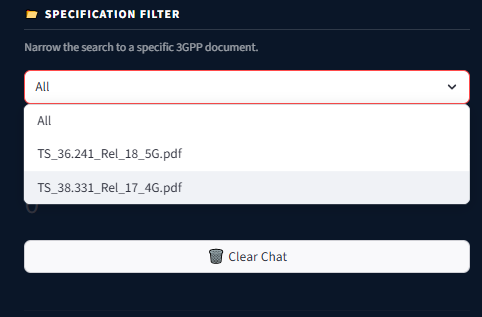
\includegraphics[width=\textwidth]{figures/chapter07/80.png}
    \caption{Specification Filter allowing users to restrict semantic retrieval to selected 3GPP Technical Specifications.}
    \label{fig:specification_filter}
\end{figure}

By eliminating unrelated specifications before semantic retrieval, metadata filtering reduces computational complexity, improves retrieval precision, and minimizes the likelihood of retrieving technically similar but contextually unrelated document sections. This filtering mechanism is particularly valuable when multiple specifications describe related procedures using similar terminology.

%%%%%%%%%%%%%%%%%%%%%%%%%%%%%%%%%%%%%%%%%%%%%%%%%%%%%%%%%%%%%%%%%%%%%%%%%%%%%%%%
\section{Hybrid Retrieval Pipeline}

After applying metadata filtering, the system performs semantic retrieval using a hybrid pipeline that combines dense vector search with neural relevance estimation. This two-stage retrieval strategy balances computational efficiency with retrieval accuracy and forms one of the key engineering contributions of the developed assistant.

Initially, the user's natural-language question is converted into a dense embedding vector using the same embedding model employed during document indexing. The generated embedding is then submitted to the Qdrant vector database, which performs Approximate Nearest Neighbor (ANN) search to retrieve the Top-K semantically similar document chunks.

Instead of directly forwarding these retrieved chunks to the language model, the proposed system performs an additional refinement stage to improve retrieval quality. This refinement reduces redundant context, removes partially relevant passages, and prioritizes document chunks that best answer the user's question.

Figure~\ref{fig:retrieval_pipeline} presents the execution stages displayed during query processing.

\begin{figure}[H]
    \centering
    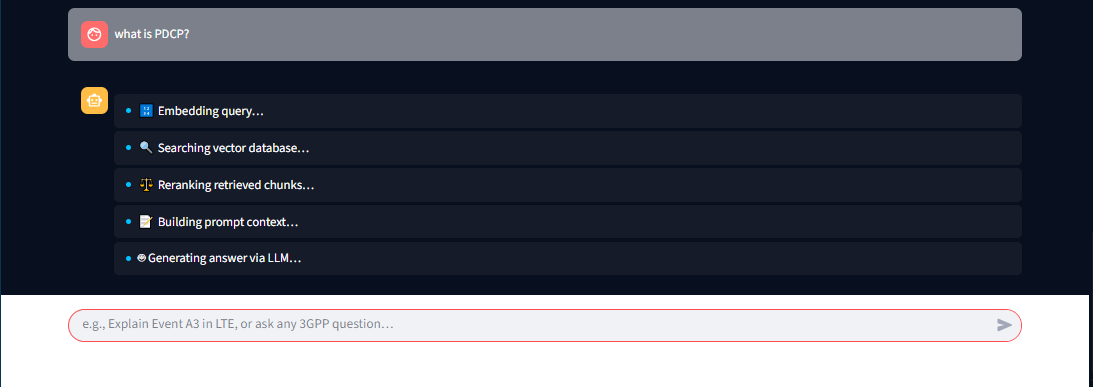
\includegraphics[width=\textwidth]{figures/chapter07/5.png}
    \caption{Execution stages of the hybrid Retrieval-Augmented Generation pipeline.}
    \label{fig:retrieval_pipeline}
\end{figure}

The implemented retrieval pipeline consists of the following stages:

\begin{enumerate}

\item Query embedding generation.

\item Metadata-aware vector retrieval using Qdrant.

\item Duplicate chunk removal.

\item Cross Encoder semantic re-ranking.

\item Selection of the highest-ranked document chunks.

\item Prompt construction.

\item Large Language Model inference.

\end{enumerate}

This hybrid retrieval strategy significantly improves response quality compared to relying solely on dense vector similarity.

%%%%%%%%%%%%%%%%%%%%%%%%%%%%%%%%%%%%%%%%%%%%%%%%%%%%%%%%%%%%%%%%%%%%%%%%%%%%%%%%
\section{Cross Encoder Re-ranking}

Although dense vector retrieval effectively retrieves semantically related specification sections, the retrieved candidate chunks may still contain partially relevant information. To improve retrieval precision, the Telecom RAG Assistant incorporates a Cross Encoder re-ranking stage before prompt construction.

Unlike embedding models that independently encode the query and document, a Cross Encoder jointly processes both inputs within the same neural network. This architecture enables the model to analyze complex semantic relationships between the user query and each retrieved document chunk, producing a highly accurate relevance score.

Following the initial retrieval stage, every candidate chunk retrieved from Qdrant is evaluated by the Cross Encoder. The model computes an independent relevance score for every query-document pair, after which the retrieved chunks are sorted according to their semantic relevance.

Only the highest-ranked chunks are selected for inclusion within the final prompt supplied to the language model. Consequently, the prompt contains highly relevant engineering context while excluding redundant or weakly related information.

This additional neural re-ranking stage substantially improves the factual accuracy of the generated responses by ensuring that the language model receives only the most informative specification excerpts.

%%%%%%%%%%%%%%%%%%%%%%%%%%%%%%%%%%%%%%%%%%%%%%%%%%%%%%%%%%%%%%%%%%%%%%%%%%%%%%%%
\section{Prompt Construction}

Prompt construction represents the final stage before invoking the Large Language Model. Rather than forwarding only the user's question, the system constructs a structured prompt that combines the retrieved specification context with carefully designed system instructions.

The prompt consists of three principal components:

\begin{enumerate}

\item A system prompt defining the assistant's behavior and restricting responses to the retrieved engineering context.

\item The highest-ranked specification chunks obtained after semantic retrieval and Cross Encoder re-ranking.

\item The user's original engineering question.

\end{enumerate}

The system prompt explicitly instructs the language model to generate responses exclusively from the supplied specification excerpts. Whenever the retrieved context does not contain sufficient information to answer the user's question, the model is instructed to acknowledge the absence of supporting evidence rather than generating speculative or hallucinated information.

The retrieved document chunks preserve their original metadata throughout the prompt construction process. Consequently, the generated response can include references to the corresponding Technical Specification number, release version, section identifier, and page number.

This prompt engineering strategy enables the Telecom RAG Assistant to produce responses that are both conversational and technically reliable while maintaining complete traceability to the original engineering documentation.
%%%%%%%%%%%%%%%%%%%%%%%%%%%%%%%%%%%%%%%%%%%%%%%%%%%%%%%%%%%%%%%%%%%%%%%%%%%%%%%%
\section{LLM Response Generation}

After the prompt has been constructed, it is transmitted to the selected Large Language Model (LLM) through the OpenRouter API. Unlike conventional conversational AI systems that rely solely on the model's internal knowledge, the Telecom RAG Assistant generates responses exclusively from the contextual information retrieved from the indexed 3GPP Technical Specifications.

The prompt supplied to the LLM consists of three main components:

\begin{enumerate}
    \item System instructions that define the assistant's role and constrain its behaviour.
    \item The retrieved specification chunks selected after semantic retrieval and Cross Encoder re-ranking.
    \item The user's original engineering question.
\end{enumerate}

The system prompt explicitly instructs the model to answer only using the supplied engineering context. Whenever sufficient information cannot be found within the retrieved specification excerpts, the assistant is instructed to acknowledge the absence of evidence rather than generating speculative information. This prompt engineering strategy significantly reduces hallucination and improves the reliability of generated responses.

After inference, the generated answer is returned together with the supporting references corresponding to the retrieved document chunks. Each response therefore remains directly traceable to the original 3GPP specification, allowing engineers to verify every statement against the official standard.

Figure~\ref{fig:event_a3_answer} illustrates a generated response describing the LTE Event A3 measurement event.

\begin{figure}[H]
    \centering
    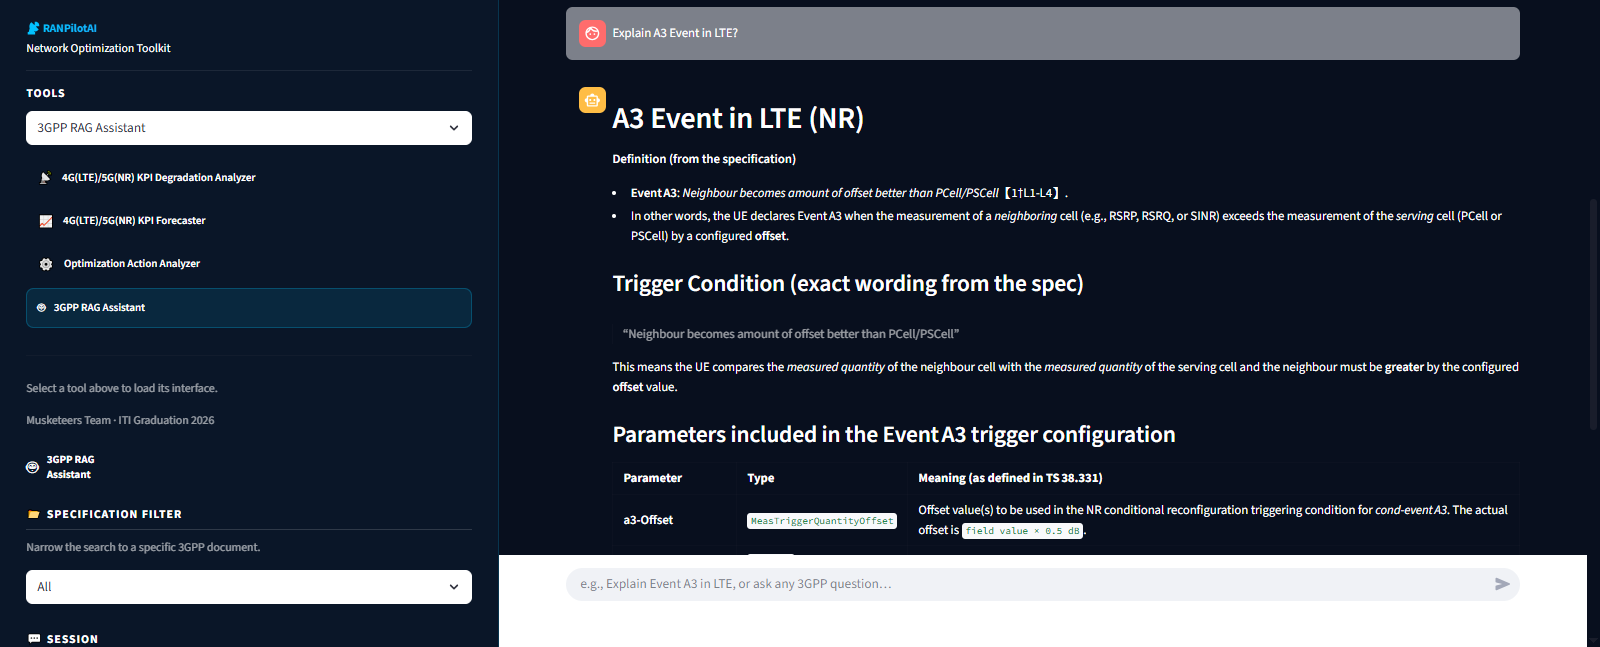
\includegraphics[width=\textwidth]{figures/chapter07/1.png}
    \caption{Generated engineering response for the LTE Event A3 measurement event.}
    \label{fig:event_a3_answer}
\end{figure}

The generated response contains both explanatory text and structured engineering information, allowing engineers to understand the underlying protocol behavior without manually navigating multiple specification sections.

%%%%%%%%%%%%%%%%%%%%%%%%%%%%%%%%%%%%%%%%%%%%%%%%%%%%%%%%%%%%%%%%%%%%%%%%%%%%%%%%
\section{User Interface}

The Telecom RAG Assistant provides an interactive graphical user interface developed using Streamlit. The interface was designed to simplify interaction with complex engineering documentation while exposing the internal stages of the Retrieval-Augmented Generation pipeline.

The main interface consists of four principal components:

\begin{itemize}
    \item Module navigation panel.
    \item Specification filtering controls.
    \item Conversational chat interface.
    \item Supporting citation viewer.
\end{itemize}

The conversational interface enables engineers to formulate technical questions using natural language instead of manually searching specification documents.

Figure~\ref{fig:main_ui} presents the main interface of the Telecom RAG Assistant.

\begin{figure}[H]
    \centering
    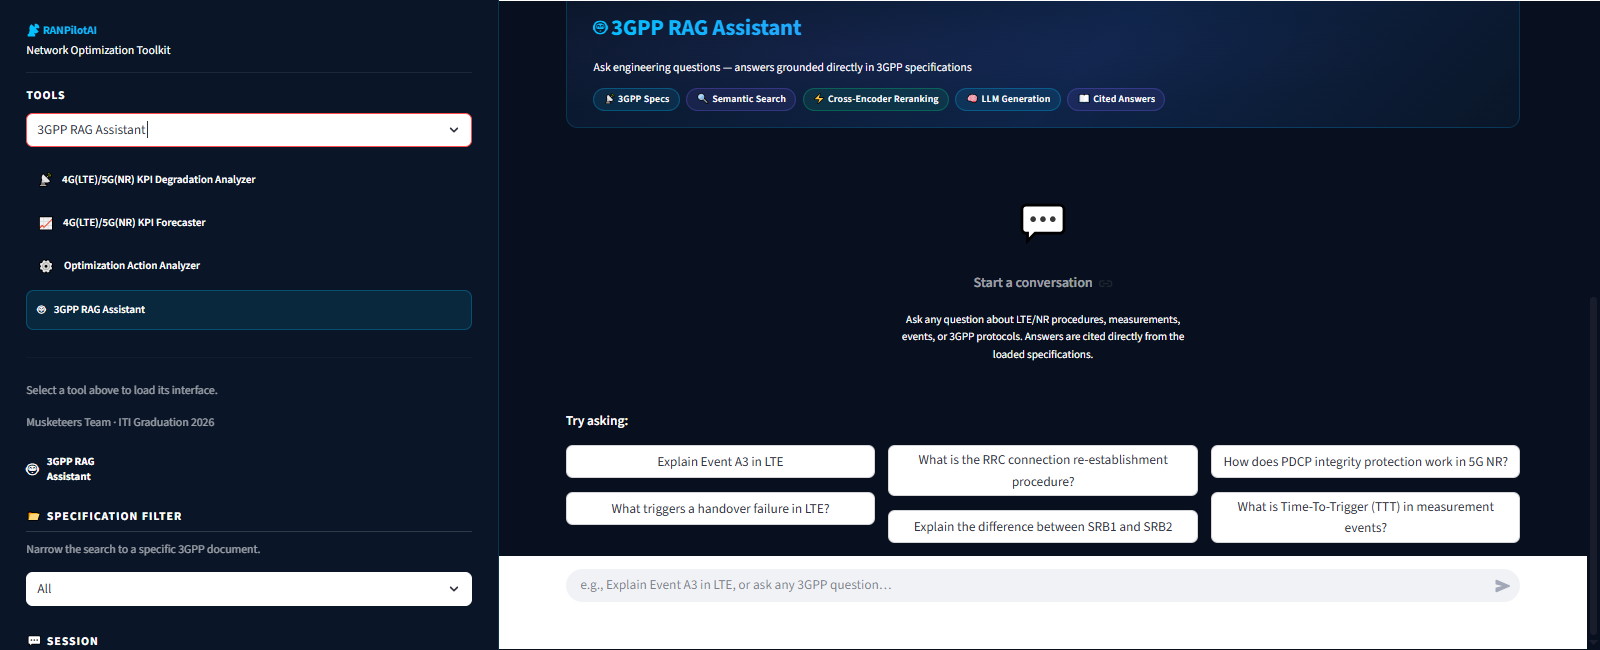
\includegraphics[width=\textwidth]{figures/chapter07/11.png}
    \caption{Main interface of the Telecom RAG Assistant.}
    \label{fig:main_ui}
\end{figure}



One of the key capabilities of the developed Telecom RAG Assistant is its ability to maintain conversational context across successive user interactions. Rather than treating each query as an isolated request, the assistant leverages the previous questions and responses within the ongoing conversation to better interpret follow-up queries. This contextual awareness enables engineers to ask natural continuation questions without repeatedly providing the complete technical context, resulting in a more intuitive and efficient interaction.
For example, after requesting an explanation of a specific LTE or NR procedure, the user may ask a follow-up question using pronouns or abbreviated terminology, and the assistant is able to infer the intended context from the conversation history before retrieving the most relevant specification excerpts. This conversational capability closely resembles the workflow of human technical discussions and significantly improves the usability of the system during troubleshooting and standards exploration.
\vspace{3mm}
Figure~\ref{fig:ho_conn_answer} 
illustrates an example in which the assistant correctly interprets a follow-up question regarding the \texttt{HO-Conn} field by utilizing the context established in the previous interaction. The generated response remains grounded in the retrieved 3GPP specifications while preserving conversational continuity, allowing engineers to explore related concepts naturally without restarting the search process.


\begin{figure}[H]
    \centering
    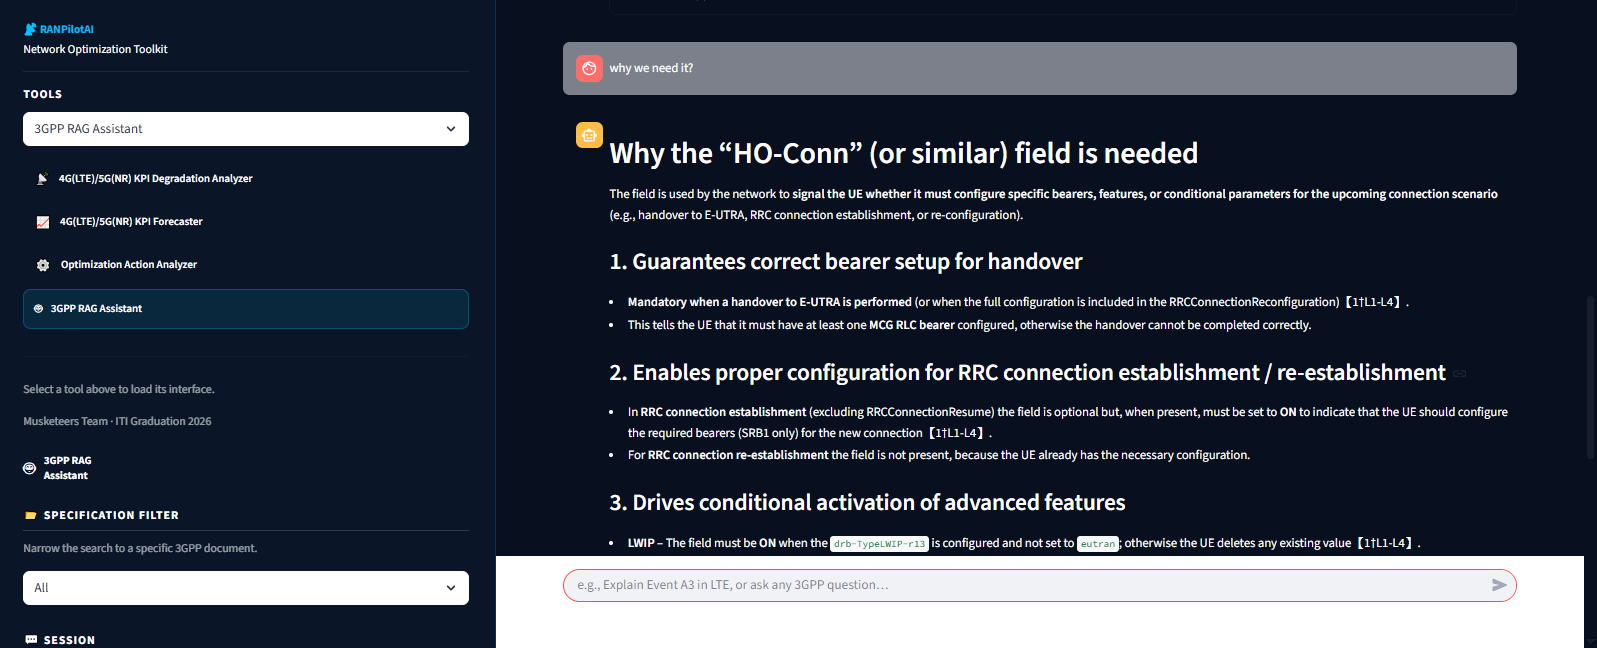
\includegraphics[width=\textwidth]{figures/chapter07/3.png}
    \caption{Context-aware response generated by the Telecom RAG Assistant using information from previous user interactions within the same conversation.}
    \label{fig:ho_conn_answer}
\end{figure}

The assistant also produces concise engineering summaries highlighting the most important technical points extracted from the specifications.

\begin{figure}[H]
    \centering
    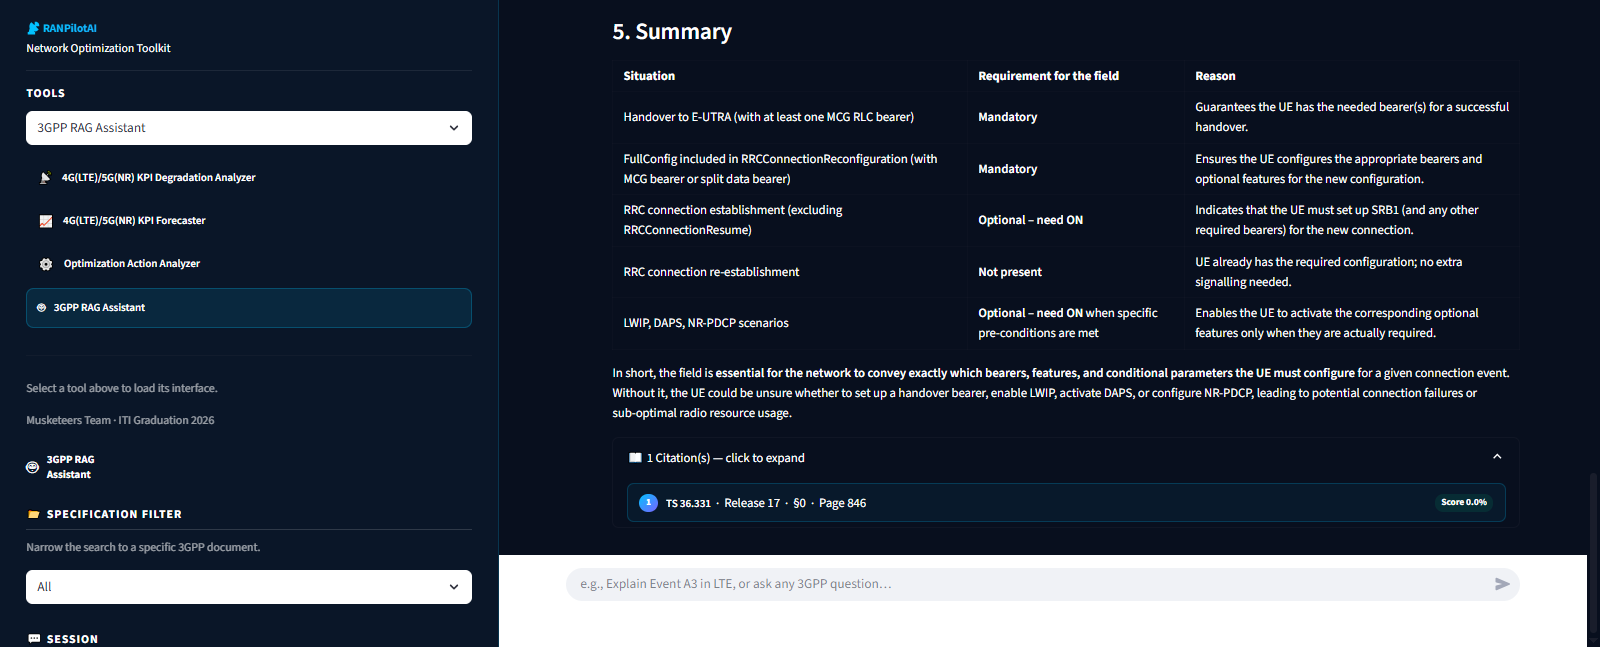
\includegraphics[width=\textwidth]{figures/chapter07/4.png}
    \caption{Structured engineering summary generated by the Telecom RAG Assistant.}
    \label{fig:summary_response}
\end{figure}

The developed assistant is capable of interpreting engineering tables directly from the indexed specifications.

Figure~\ref{fig:pdcp_answer} illustrates an example response describing the Packet Data Convergence Protocol (PDCP), while Figure~\ref{fig:pdcp_summary} presents the corresponding engineering summary generated from the retrieved specification sections.

\begin{figure}[H]
    \centering
    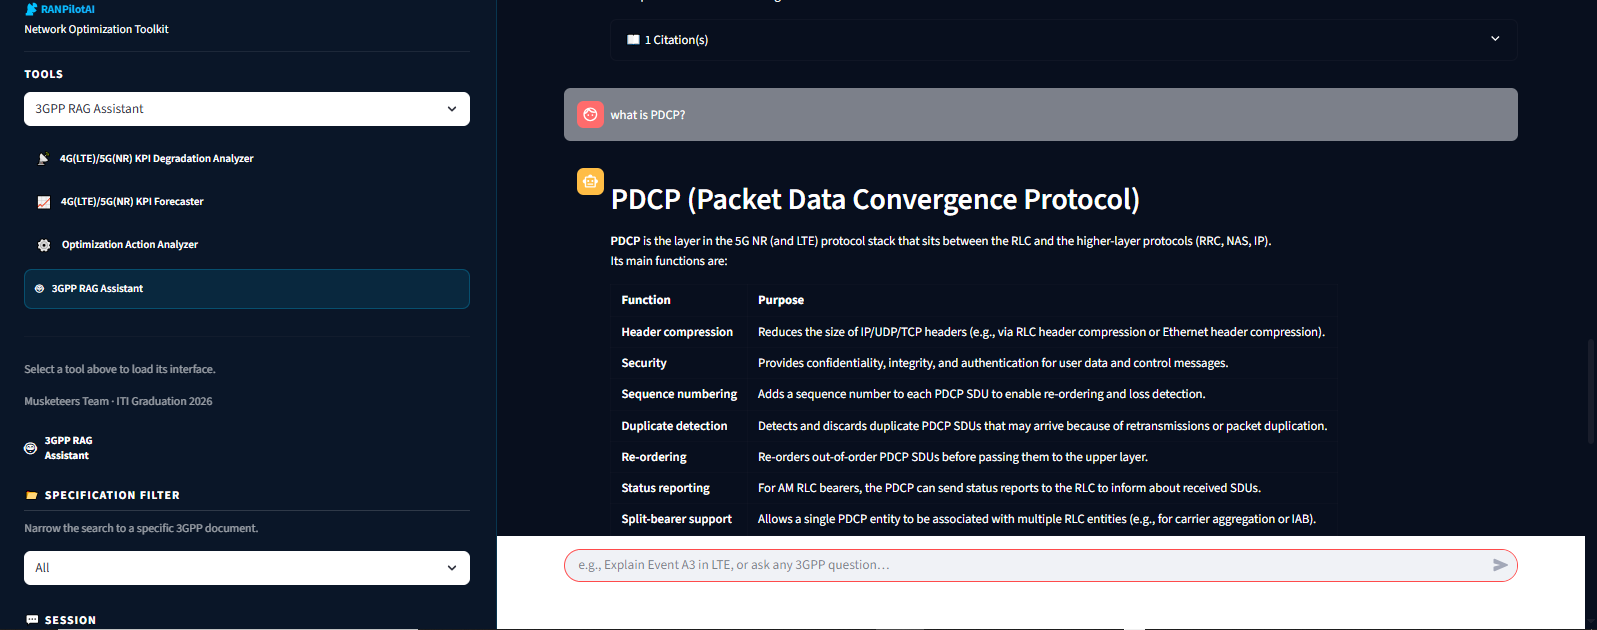
\includegraphics[width=\textwidth]{figures/chapter07/6.png}
    \caption{Generated response explaining the Packet Data Convergence Protocol (PDCP).}
    \label{fig:pdcp_answer}
\end{figure}

\begin{figure}[H]
    \centering
    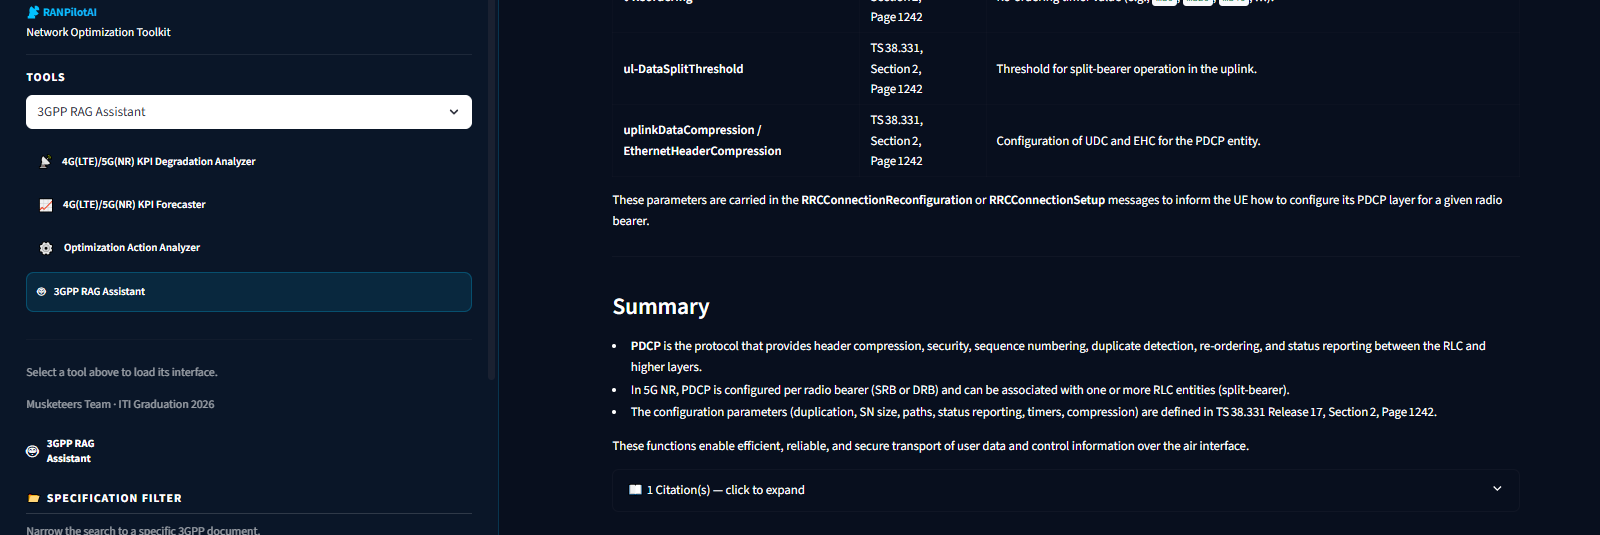
\includegraphics[width=\textwidth]{figures/chapter07/7.png}
    \caption{Structured engineering summary for the PDCP protocol.}
    \label{fig:pdcp_summary}
\end{figure}

The interface automatically attaches supporting citations to every generated response, allowing engineers to verify the retrieved information directly from the corresponding Technical Specification.

%%%%%%%%%%%%%%%%%%%%%%%%%%%%%%%%%%%%%%%%%%%%%%%%%%%%%%%%%%%%%%%%%%%%%%%%%%%%%%%%
\section{Performance Evaluation}

The developed Telecom RAG Assistant incorporates an integrated profiling mechanism that records the execution time of every stage within the Retrieval-Augmented Generation pipeline. This profiling framework assists developers in identifying computational bottlenecks while providing transparency regarding the internal processing workflow.

For every submitted query, the profiler measures:

\begin{itemize}
    \item Query embedding time.
    \item Vector database retrieval time.
    \item Cross Encoder re-ranking time.
    \item Prompt construction time.
    \item Large Language Model inference time.
    \item Total response latency.
\end{itemize}

Figure~\ref{fig:performance_logs} illustrates the execution statistics generated during query processing.

\begin{figure}[H]
    \centering
    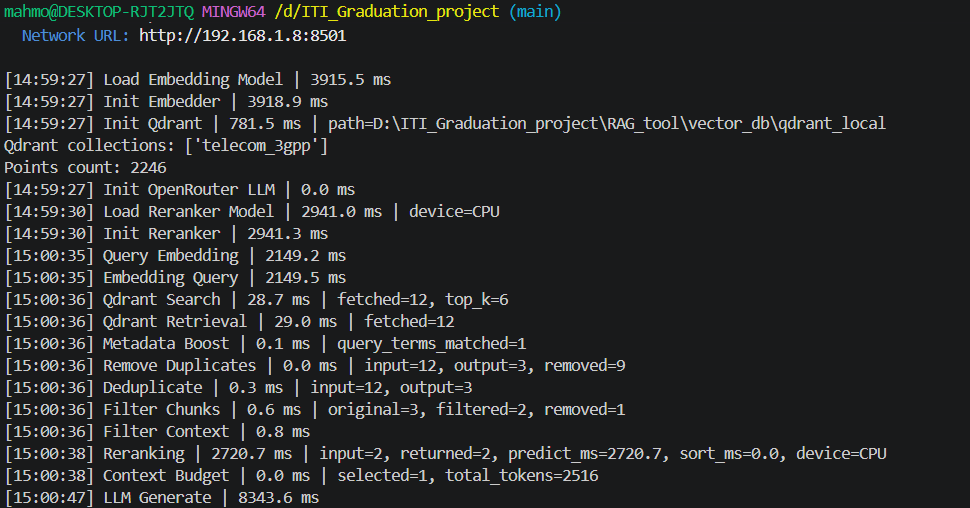
\includegraphics[width=\textwidth]{figures/chapter07/9.png}
    \caption{Pipeline profiling and execution statistics generated during query processing.}
    \label{fig:performance_logs}
\end{figure}

The collected execution statistics provide valuable insight into the computational cost of each pipeline stage and facilitate future optimization of the retrieval and inference process.

%%%%%%%%%%%%%%%%%%%%%%%%%%%%%%%%%%%%%%%%%%%%%%%%%%%%%%%%%%%%%%%%%%%%%%%%%%%%%%%%
\section{Discussion}

The developed Telecom RAG Assistant successfully demonstrates how Retrieval-Augmented Generation can be adapted to the telecommunications domain through the integration of semantic retrieval, metadata-aware filtering, neural re-ranking, and conversational language models. By grounding every generated response in official 3GPP Technical Specifications, the system significantly reduces hallucination while maintaining complete traceability to the original engineering documentation.

Compared with traditional PDF searching, the proposed assistant provides a more intuitive interaction model that enables engineers to obtain accurate technical explanations using natural language. The modular architecture further simplifies future extensions, allowing additional specifications, embedding models, or language models to be incorporated with minimal modifications to the overall system.

%%%%%%%%%%%%%%%%%%%%%%%%%%%%%%%%%%%%%%%%%%%%%%%%%%%%%%%%%%%%%%%%%%%%%%%%%%%%%%%%
\section{Limitations}

Although the developed Telecom RAG Assistant provides accurate and traceable engineering responses, several limitations remain.

The quality of generated responses depends directly on the availability and completeness of the indexed Technical Specifications. Information that has not been indexed cannot be retrieved by the system.

Additionally, the overall response latency is influenced by the selected embedding model, vector database search, Cross Encoder inference, and external Large Language Model response time. Processing very large document collections may therefore require additional optimization or distributed deployment strategies.

Finally, although Retrieval-Augmented Generation substantially reduces hallucination, complete elimination of incorrect responses cannot be guaranteed under all operating conditions.

%%%%%%%%%%%%%%%%%%%%%%%%%%%%%%%%%%%%%%%%%%%%%%%%%%%%%%%%%%%%%%%%%%%%%%%%%%%%%%%%
\section{Future Improvements}

Several enhancements can further improve the proposed Telecom RAG Assistant.

Future work includes supporting additional telecommunication standards beyond LTE and 5G NR, integrating multimodal retrieval capable of interpreting engineering figures and diagrams, incorporating continuous indexing of newly released 3GPP specifications, and evaluating larger domain-specific embedding models.

Future versions may also integrate local Large Language Models to reduce dependency on external inference services while improving privacy and deployment flexibility.

%%%%%%%%%%%%%%%%%%%%%%%%%%%%%%%%%%%%%%%%%%%%%%%%%%%%%%%%%%%%%%%%%%%%%%%%%%%%%%%%
\section{Chapter Summary}

This chapter presented the design and implementation of the Telecom RAG Assistant developed as part of the RANPilotAI platform. Beginning with the motivation and theoretical foundations of Retrieval-Augmented Generation, the chapter described the complete processing pipeline including PDF processing, section-aware chunking, embedding generation, vector storage, metadata filtering, hybrid semantic retrieval, Cross Encoder re-ranking, prompt construction, and language model inference.
The implementation demonstrates how modern Artificial Intelligence techniques can be combined with official 3GPP Technical Specifications to provide an intelligent engineering assistant capable of answering complex telecommunication questions with high accuracy and complete source traceability. The presented architecture establishes a practical foundation for AI-assisted standards consultation and represents an important step toward intelligent engineering support systems for future mobile communication networks.